\documentclass[11pt]{article}
\usepackage[margin=0.85in]{geometry}
\usepackage{enumitem}
\usepackage{booktabs}
\usepackage{amsmath}
\usepackage[table]{xcolor}
\usepackage{graphicx}
\usepackage{caption}

\setlength{\parskip}{5pt}
\setlength{\parindent}{0pt}

\begin{document}

\begin{center}
{\Large\bfseries HACE: Addressing Viability Failure in Sequential RL\\[2pt]
with Homeostatic Auxiliary Rewards}\\[6pt]
{\small\color{gray} Project Brief for PI Review --- \today}
\end{center}

\vspace{-4pt}\hrule\vspace{6pt}

\textbf{Core Claim.}
Continual RL focuses on \emph{catastrophic forgetting}, but in embodied settings with shared energy, agents face a complementary failure: \textbf{viability failure}---they \emph{die before they can learn} the next task.
EWC, ER, and L2 operate on weights/data and cannot fix a survival problem.
We propose \textbf{HACE}: a task-invariant auxiliary reward $r_t^H = |H^* \!-\! E_t| - |H^* \!-\! E_{t+1}|$ that incentivizes energy management.

\textbf{Benchmark.}
12 gridworld tasks (5$\times$5 to 7$\times$7) sharing energy dynamics but varying in hazards, walls, food, gates.
3 task sequences ($\alpha$/$\beta$/$\gamma$), 2 boundary modes (reset/carryover), \textbf{9 agents}:
Task-only~(A), Energy-aware~(B), \textbf{HACE}~(C), Pure Homeo~(D), Oracle~(E), EWC~(F), L2~(G), ER~(H), \textbf{HACE+EWC}~(I).

\vspace{4pt}
\textbf{Main Result: 9-Agent Suite on $\alpha$-Carryover (10 seeds).}

\begin{figure}[h]
\centering
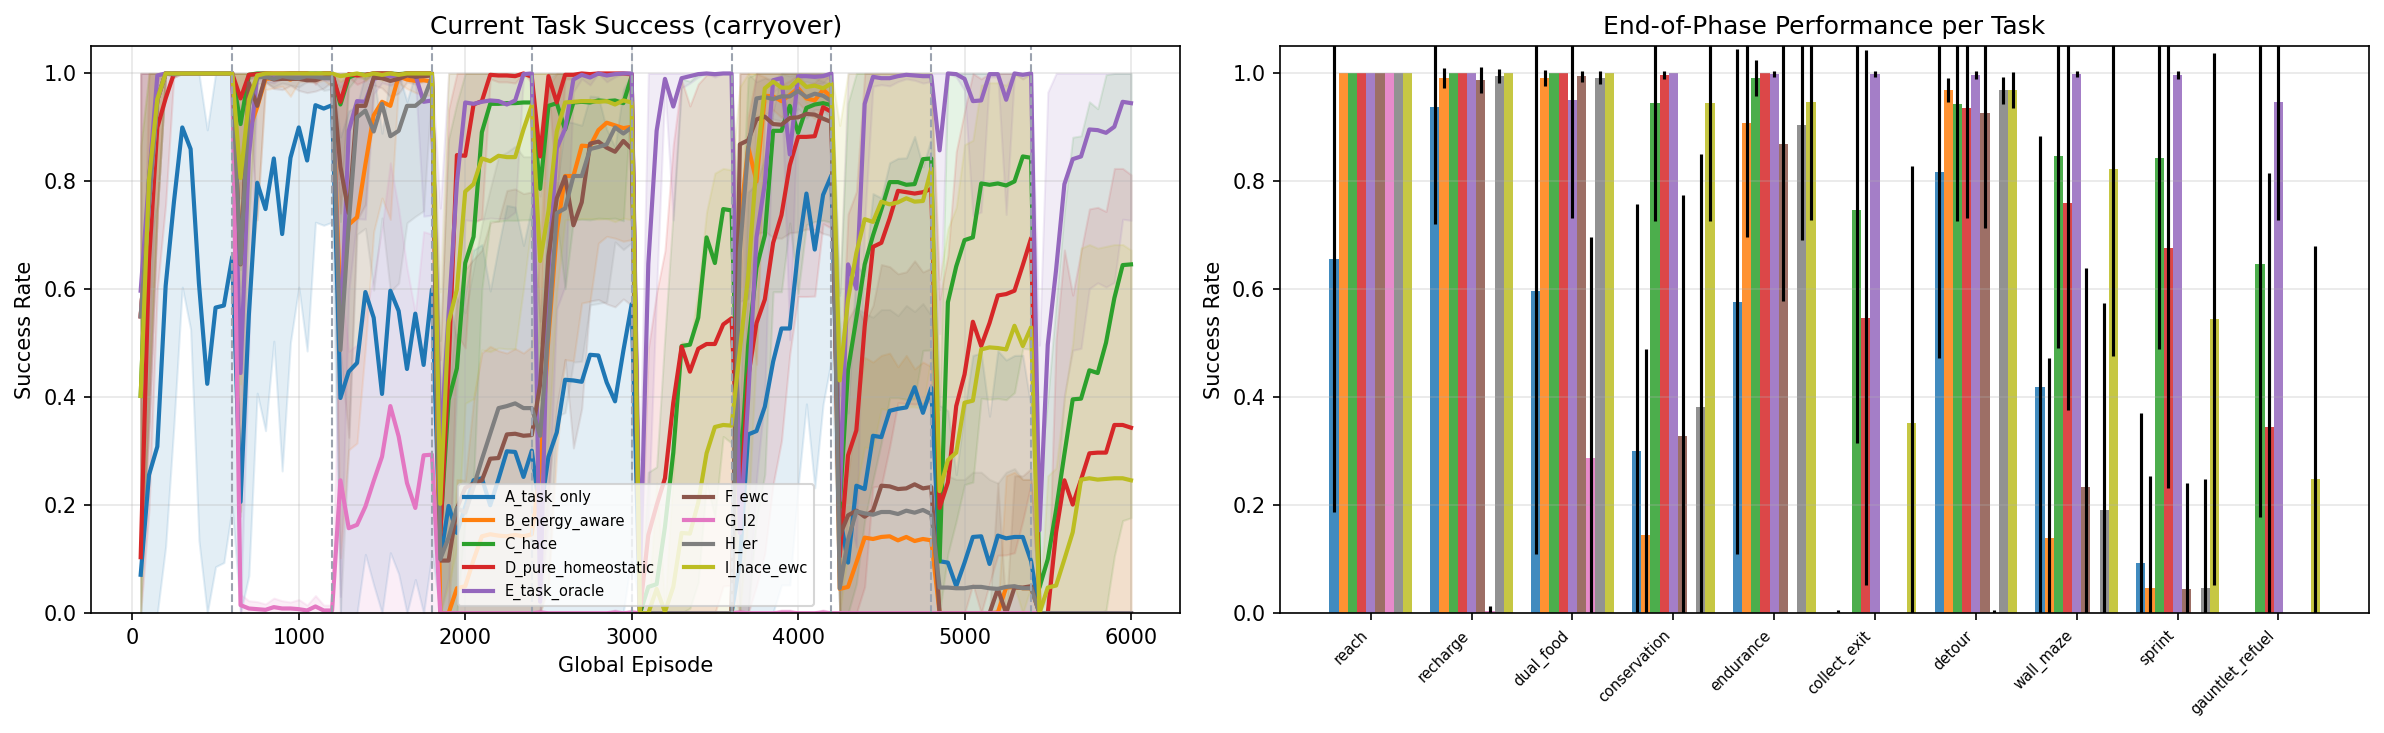
\includegraphics[width=\textwidth]{figures/e3_alpha_carryover.png}
\caption{Full 9-agent suite on the $\alpha$ sequence under carryover mode.
\emph{Left}: current-task success during training.
\emph{Right}: final retention across all 10 tasks.}
\end{figure}

\begin{table}[h]
\centering\small
\caption{Final average success, boundary solvability, and terminal energy ($\alpha$-carryover).}
\vspace{2pt}
\begin{tabular}{@{}llccc@{}}
\toprule
\textbf{ID} & \textbf{Agent} & \textbf{Avg Success} & \textbf{Boundary Solv.} & \textbf{Terminal E} \\
\midrule
A & Task-only           & 0.020 & 0.033 & 0.0 \\
B & Energy-aware        & 0.085 & 0.016 & 0.0 \\
C & \textbf{HACE (ours)} & 0.170 & \textbf{0.103} & \textbf{9.9} \\
D & Pure Homeostatic    & 0.157 & 0.080 & 5.3 \\
E & Task Oracle         & 0.261 & ---   & 15.2 \\
F & EWC                 & 0.261 & 0.033 & 0.0 \\
G & L2                  & 0.137 & 0.001 & 0.0 \\
H & ER                  & 0.249 & 0.011 & 0.0 \\
I & \textbf{HACE+EWC}   & \textbf{0.335} & \textbf{0.107} & 4.4 \\
\bottomrule
\end{tabular}
\end{table}

\textbf{Key Findings:}
\begin{enumerate}[leftmargin=*, itemsep=1pt, topsep=2pt]
\item \textbf{Viability failure is real}: A, F, G, H all end with \textbf{0.0 terminal energy}---they die at task boundaries. Boundary solvability $\leq 0.033$.
\item \textbf{CRL alone does not fix survival}: EWC~(F) matches Oracle~(E) in avg success (0.261) but has 0.0 terminal energy. It solves tasks only because eval resets energy per episode; in truly sequential deployment it would fail.
\item \textbf{HACE keeps agents alive}: HACE~(C) maintains 9.9 terminal energy and 3$\times$ higher boundary solvability than any non-homeostatic agent.
\item \textbf{HACE+EWC is best}: Agent~I achieves the highest avg success (\textbf{0.335}) \emph{and} 0.107 boundary solvability, confirming that viability (HACE) and forgetting (EWC) are \textbf{orthogonal}.
\item \textbf{Hardest task}: HACE~(C) solves \texttt{gauntlet\_refuel} at 0.65 success; EWC/ER/L2 all score 0.00---only agents that conserve energy survive to reach the end.
\end{enumerate}

\vspace{4pt}
\textbf{Supporting Evidence (Earlier Experiments).}

\begin{figure}[h]
\centering
\begin{minipage}[t]{0.48\textwidth}
\centering
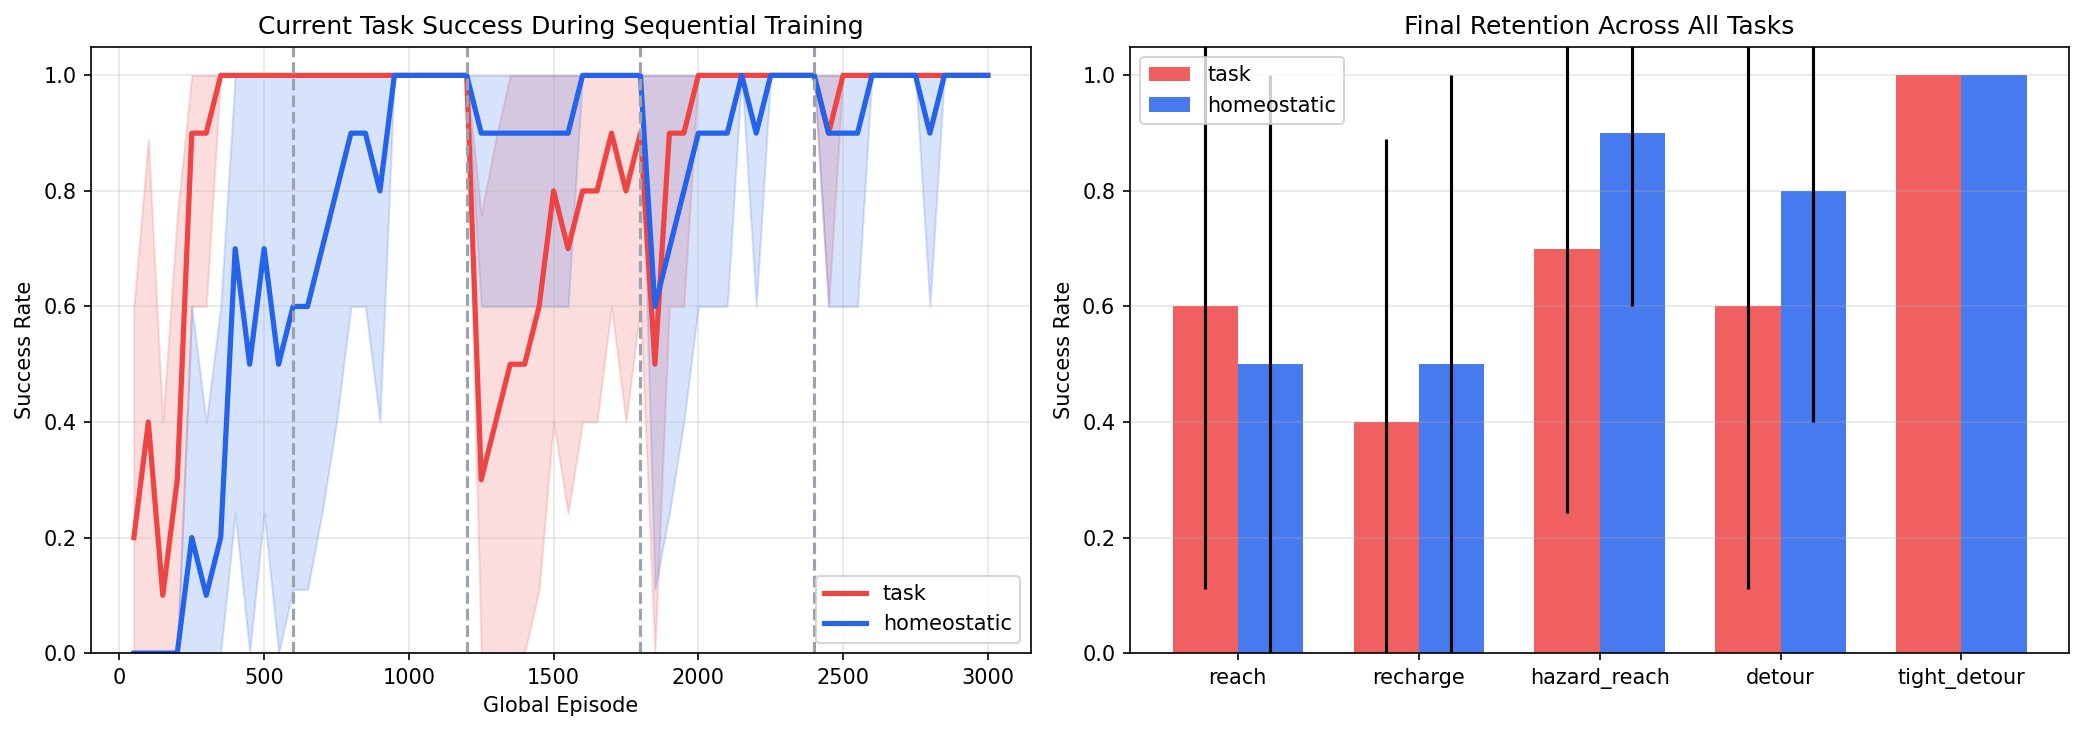
\includegraphics[width=\textwidth]{figures/sequential_pilot.png}
\caption{5-task pilot: homeostatic agent retains +20\% on later resource-dependent tasks.}
\end{minipage}\hfill
\begin{minipage}[t]{0.48\textwidth}
\centering
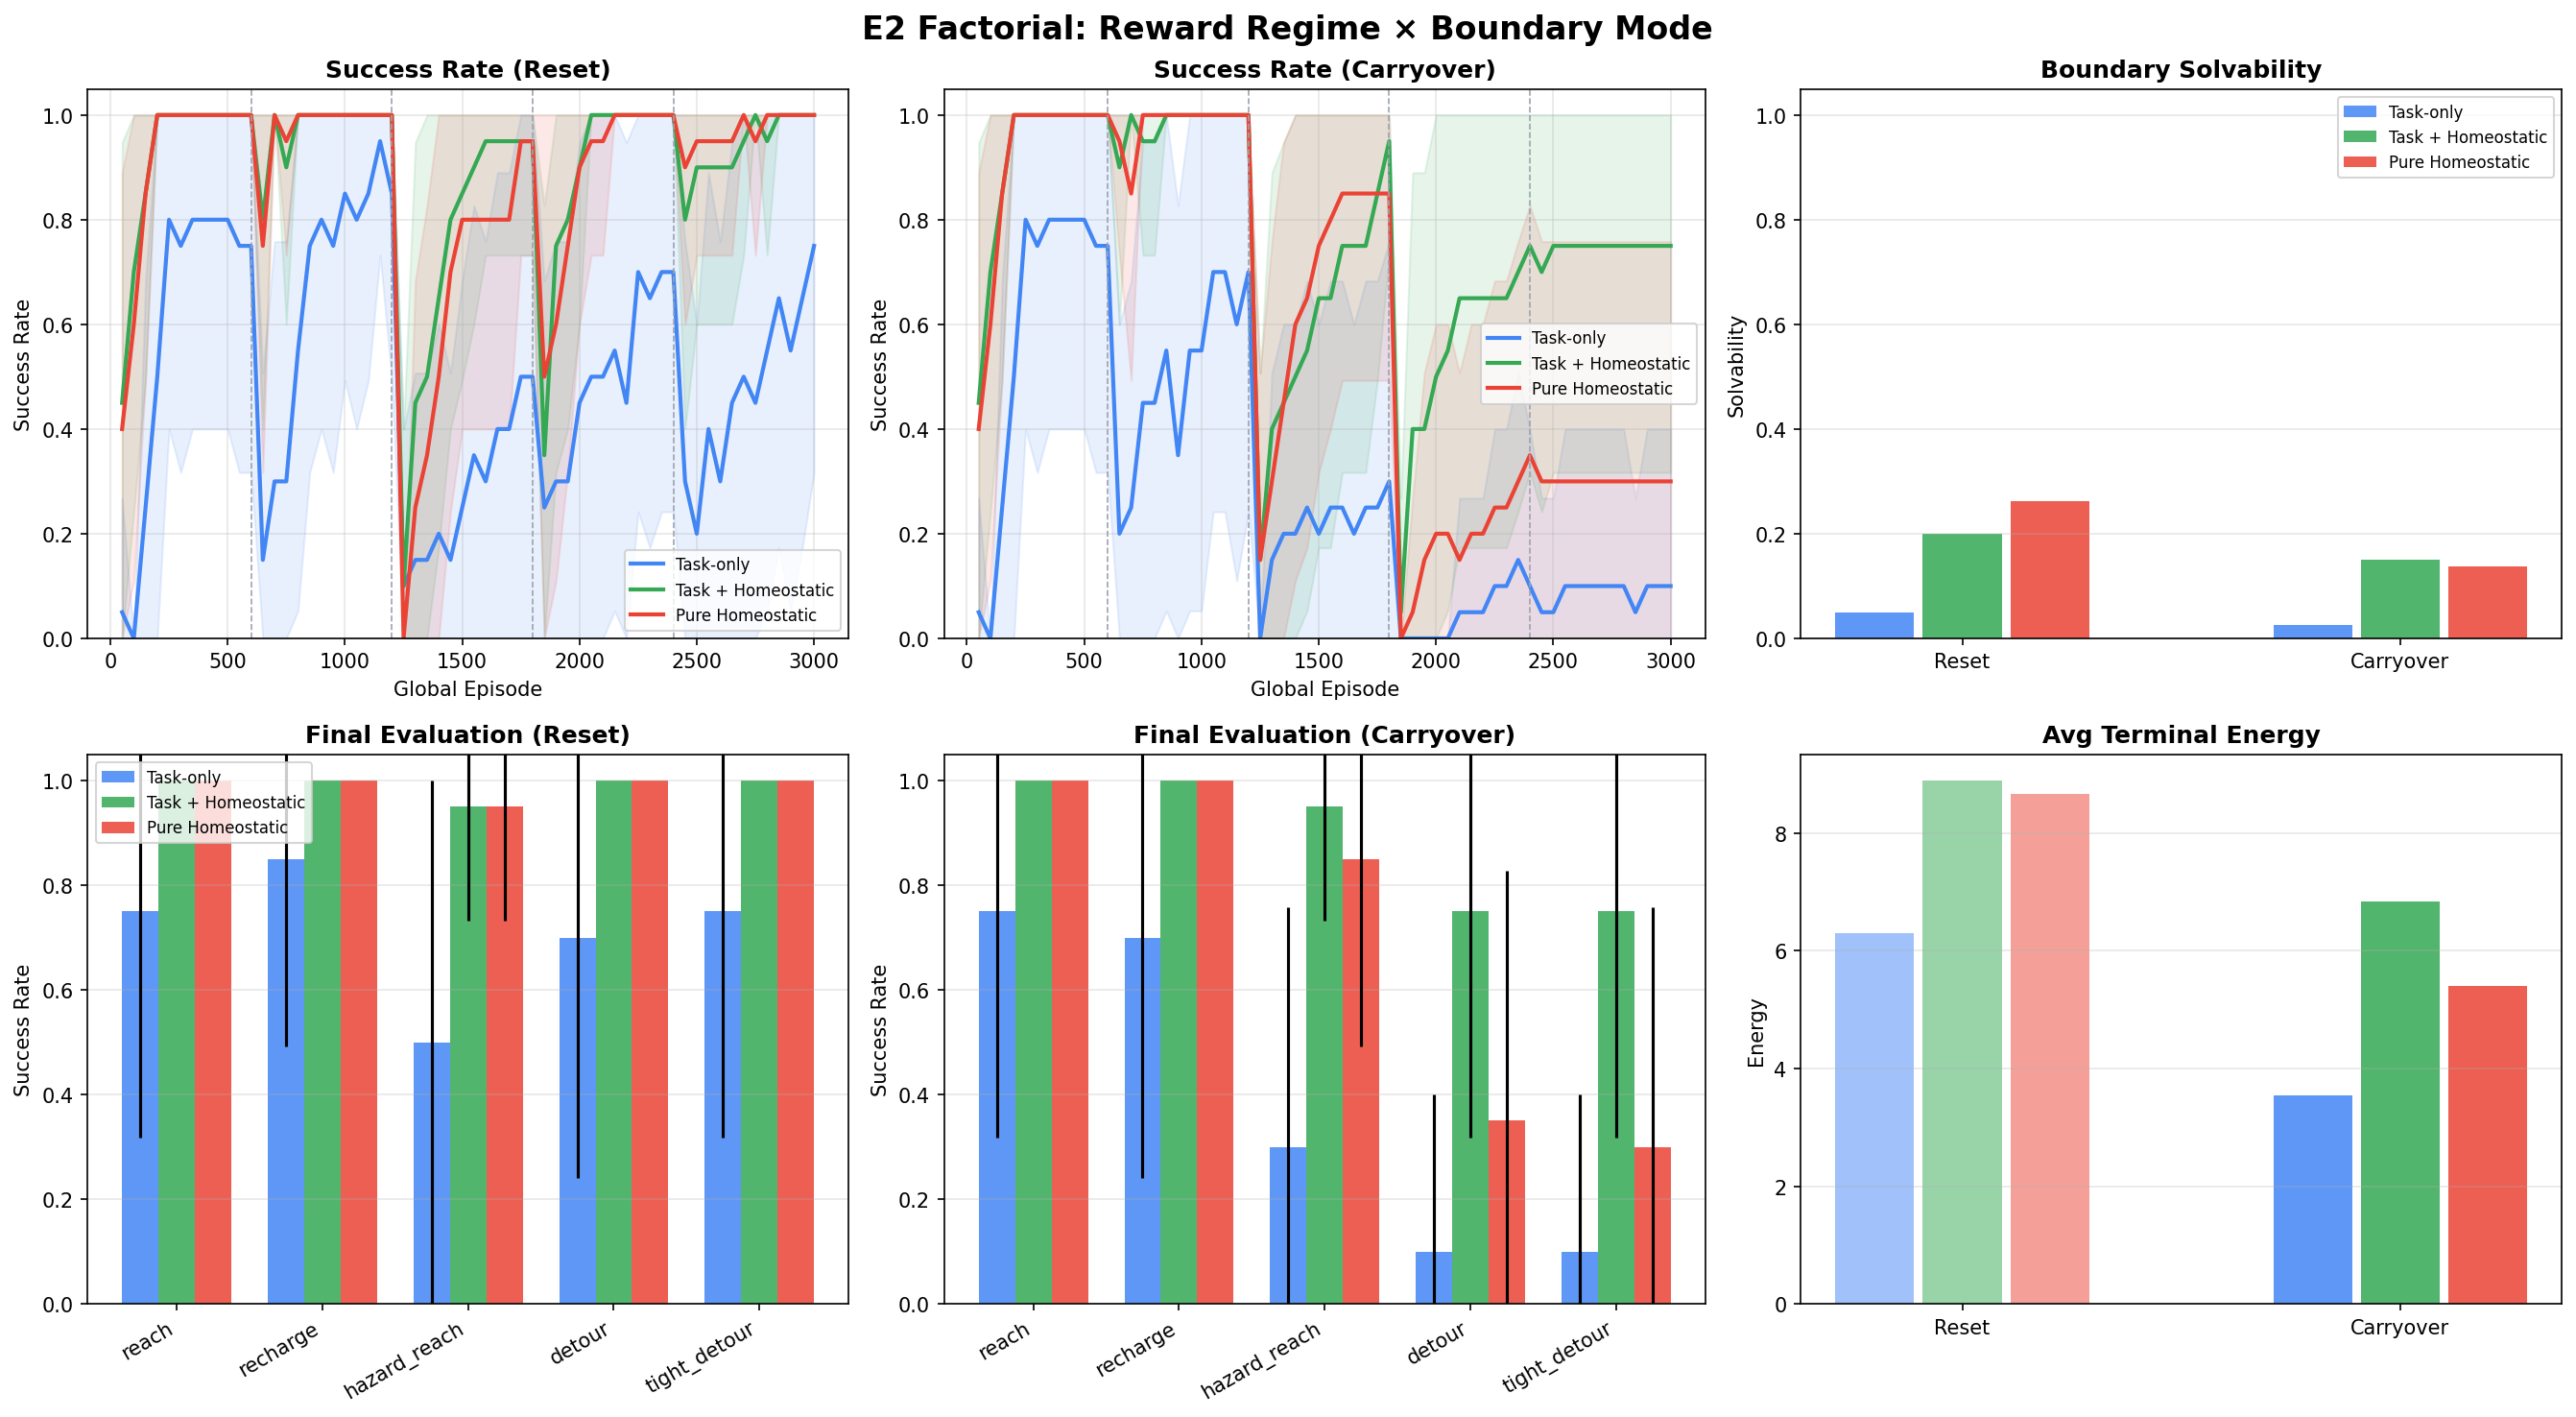
\includegraphics[width=\textwidth]{figures/e2_factorial.png}
\caption{Factorial: task-only collapses to 0.1 under carryover; same weights work under reset $\Rightarrow$ not forgetting.}
\end{minipage}
\end{figure}

\vspace{4pt}
\textbf{Done vs.\ TODO.}

\begin{table}[h]
\small\centering
\begin{tabular}{@{}lll@{}}
\toprule
& \textbf{Done} & \textbf{TODO} \\
\midrule
Environment & 12 tasks, 3 sequences, 2 modes & --- \\
Agents      & All 9 implemented & --- \\
Exp: Full suite & $\alpha$-carryover, 9 agents, 10 seeds & $\beta$/$\gamma$ sequences + reset mode \\
Exp: Pilot + Factorial & Complete, multi-seed & --- \\
Statistics  & Descriptive & Holm-Bonferroni, bootstrap CI \\
Controls    & --- & Sham / permutation controls \\
Ablations   & --- & $\alpha$ sensitivity, step cost \\
\bottomrule
\end{tabular}
\end{table}

\textbf{Questions for PI.}
\begin{enumerate}[leftmargin=*, itemsep=1pt, topsep=2pt]
\item \textbf{The Core Problem}: We found that standard RL agents simply die when energy carries over between tasks. Is this evidence strong enough to convince reviewers that current RL benchmarks are ignoring a critical ``survival'' problem?
\item \textbf{Absolute vs. Relative Performance}: Our method (HACE) survives when others die, but its average task success rate is still somewhat low (0.170). Is this absolute low number a dealbreaker for publication, or is the stark contrast in survival (terminal energy 9.9 vs 0.0) enough?
\item \textbf{Combining Methods}: When we combine our survival reward with a standard memory method (EWC), we get the best overall results. Is this enough to proudly claim our method solves the ``staying alive'' problem while standard methods solve the ``remembering'' problem?
\item \textbf{Paper Focus}: Should we focus the entire paper purely on this new ``agents must stay alive to learn'' narrative, or do we need to balance it by analyzing how well they perform the specific gridworld tasks?
\item \textbf{Story Completeness}: Looking at our current story---agents die, our reward keeps them alive, and combining both gives the best result---does this feel like a complete, convincing paper, or are there obvious holes a reviewer will attack?
\end{enumerate}

\end{document}
